	%сделать восклицательный знак
\documentclass[a4paper,12pt,fleqn]{article} % добавить leqno в [] для нумерации слева

%%% Работа с русским языком
\usepackage{cmap}					% поиск в PDF
\usepackage{mathtext} 				% русские буквы в формулах
\usepackage[T2A]{fontenc}			% кодировка
\usepackage[utf8]{inputenc}			% кодировка исходного текста
\usepackage[english,russian]{babel}	% локализация и переносы

%%% Дополнительная работа с математикой
\usepackage{amsmath,amsfonts,amssymb,amsthm,mathtools} % AMS
\usepackage{icomma} % "Умная" запятая

%% Номера формул
%\mathtoolsset{showonlyrefs=true} % Показывать номера только у тех формул, на которые есть \eqref{} в тексте.
%\usepackage{leqno} %Нумерация формул слева

%% Шрифты
\usepackage{euscript}	 % Шрифт Евклид
\usepackage{mathrsfs} % Красивый матшрифт


%% Свои команды
\DeclareMathOperator{\sgn}{\mathop{sgn}}

%% Перенос знаков в формулах (по Львовскому)
\newcommand*{\hm}[1]{#1\nobreak\discretionary{}
{\hbox{$\mathsurround=0pt #1$}}{}}

%%% Заголовок
\author{}
\title{}
\date{}



%%% Теоремы
%\theoremstyle{definition}
%\newtheorem{case}{Задача}[section]
%\renewcommand{\thecase}{\arabic{case}}

%\theoremstyle{definition} % "Определение"
%\newtheorem{corollary}{Пункт}[case]
%\newtheorem{problem}{Задача}[section]
%\renewcommand{\thecorollary}{\asbuk{corollary}}

\usepackage{multicol} % Несколько колонок


%%% Работа с картинками
\usepackage{graphicx}  % Для вставки рисунков
\graphicspath{{images/}{images2/}}  % папки с картинками
\setlength\fboxsep{3pt} % Отступ рамки \fbox{} от рисунка
\setlength\fboxrule{1pt} % Толщина линий рамки \fbox{}
\usepackage{wrapfig} % Обтекание рисунков текстом

%%% Работа с таблицами
\usepackage{array,tabularx,tabulary,booktabs} % Дополнительная работа с таблицами
\usepackage{longtable}  % Длинные таблицы
\usepackage{multirow} % Слияние строк в таблице

%%% Страница
%\usepackage{extsizes} % Возможность сделать 14-й шрифт
\usepackage{geometry} % Простой способ задавать поля
\geometry{top=20mm}
\geometry{bottom=20mm}
\geometry{left=30mm}
\geometry{right=20mm}
%
\usepackage{fancyhdr} % Колонтитулы
\pagestyle{fancy}
\renewcommand{\headrulewidth}{0.1mm}  % Толщина линейки, отчеркивающей верхний колонтитул
%\lfoot{Нижний левый}
%\rfoot{Нижний правый}
\rhead{Глава \thesection}
%\chead{Верхний в центре}
%\lhead{}
% \cfoot{Нижний в центре} % По умолчанию здесь номер страницы

\usepackage{setspace} % Интерлиньяж
%\onehalfspacing % Интерлиньяж 1.5
%\doublespacing % Интерлиньяж 2
%\singlespacing % Интерлиньяж 1

\usepackage{soulutf8} % Модификаторы начертания
\usepackage{bm} % Модификатор начертания для математики

%\usepackage{tikz} % Работа с графикой
%\usepackage{pgfplots}
%\usepackage{pgfplotstable}
%\usepackage[utf8]{inputenc}
%\usetikzlibrary{arrows}


\usepackage{hyperref}
\usepackage[usenames,dvipsnames,svgnames,table,rgb]{xcolor}
\hypersetup{				% Гиперссылки
	unicode=true,           % русские буквы в раздела PDF
	pdftitle={Заголовок},   % Заголовок
	pdfauthor={Автор},      % Автор
	pdfsubject={Тема},      % Тема
	pdfcreator={Создатель}, % Создатель
	pdfproducer={Производитель}, % Производитель
	pdfkeywords={keyword1} {key2} {key3}, % Ключевые слова
	colorlinks=true,       	% false: ссылки в рамках; true: цветные ссылки
	linkcolor=blue!55!red,          % внутренние ссылки
	citecolor=green,        % на библиографию
	filecolor=magenta,      % на файлы
	urlcolor=blue          % на URL
} 
\usepackage{datetime}
\newdateformat{onlyyear}{\THEYEAR}
\newdateformat{defaultdate}{\THEDAY~\monthname[\THEMONTH] \THEYEAR~г.}

\usepackage{multicol} % Несколько колонок

\usepackage{indentfirst} % Красная строка

\usepackage{tikz} % Работа с графикой
\usepackage{pgfplots} %взять данные из соседнего файла и построить по ним что-либо
\usepackage{pgfplotstable}
\usetikzlibrary{fadings}
\usetikzlibrary{decorations}
\usepgflibrary{decorations.pathmorphing}

\tikzfading[name=fade out, inner color=transparent!0,
outer color=transparent!100]

\usepackage[utf8]{inputenc}
\usetikzlibrary{arrows}
\usepackage{tcolorbox}
\usepackage{lipsum}
\tcbuselibrary{breakable}

%\usetikzlibrary{calc}

\usepackage{xparse}
\NewDocumentCommand{\definition}{mm}{ \textbf{Определение.} \textit{#1} --- #2 \vspace{0.3cm}}

\renewcommand{\familydefault}{\sfdefault}
\usepackage{float}

\usepackage{relsize}
\newcommand{\bigem}[1][1]{\text{\larger[#1]{\color{blue!55!red}{ \textbf{$ ! $}}}}}


\begin{document} % конец преамбулы, начало документа
	
\tableofcontents

\newpage


\section{Угрозы в области физической безопасности}

\begin{tcolorbox}[colback=blue!40!red!10!,colframe=blue!40!red]

В результате изучения главы студент должен \textbf{знать} основные угрозы в области обеспечения физической безопасности предприятия в сферах защиты жизни и здоровья физических лиц, обеспечения сохранности финансовых и иных материальных ценностей, а также объектов недвижимости; \textbf{уметь} сопоставлять основные угрозы с типовыми мерами обеспечения физической защиты бизнеса; \textbf{владеть} методами обеспечения физической безопасности предприятия с применением различных типов защиты, а также расчетом экономических показателей себестоимости различных вариантов охраны.

\end{tcolorbox}


\subsection{Угроза жизни и здоровью физических лиц}

Важным \textit{условием успешного функционирования любого предприятия на рынке} является защита от возникающих угроз, среди которых особую опасность представляют незаконные действия физических лиц. Последствия их действий непредсказуемы: от хищения имущества до создания чрезвычайных ситуаций на объекте. В этих условиях безопасность любого субъекта рынка осуществляется на основе принципов «разумной достаточности», «эффективность – стоимость», а также разработанной в теории и применяемой на практике концепции физической безопасности предприятия.

В рамках единой политики безопасности организации физическая безопасность является основным структурным элементом, направленным на сохранение собственности, жизни и здоровья персонала, финансовых ресурсов.\\

\definition{Физическая безопасность организации} {совокупность правовых норм, организационных мер и инженерно-технических решений, направленных на защиту важных интересов и ресурсов предприятия (объекта) от угроз злоумышленных противоправных действий физических лиц (нарушителей или злоумышленников).}

Как правило, она включает в себя силы подразделений безопасности и охраны объекта, комплекс инженерно-технических средств охраны, а также режим, установленный на объекте. Система физической защиты не должна препятствовать нормальному функционированию организации, ее технологическим процессам.

Угрозы в области физической безопасности существенно различаются по своей тяжести и зависят от возможностей и способностей нарушителя. В качестве \textit{основных видов угроз в области физической безопасности} принято различать  (см. рисунок \ref{image1}): 

\begin{itemize}
	\item Чрезвычайные ситуации (пожар, разрушение, затопление, авария, хищение опасных веществ, массовые инфекционные заболевания и отравления людей и т.п.);
	\item Промышленный шпионаж;
	\item Угрозы физическому лицу (сотрудникам): причинение вреда здоровью, причинение увечий, создание угроз для жизни;
	\item Хищение или порча имущества;
	\item Несанкционированный съем информации, содержащей государственную, служебную или коммерческую тайны;
	\item Снижение эффективности функционирования и устойчивости развития предприятия.
\end{itemize}

\begin{figure}
	\centering
	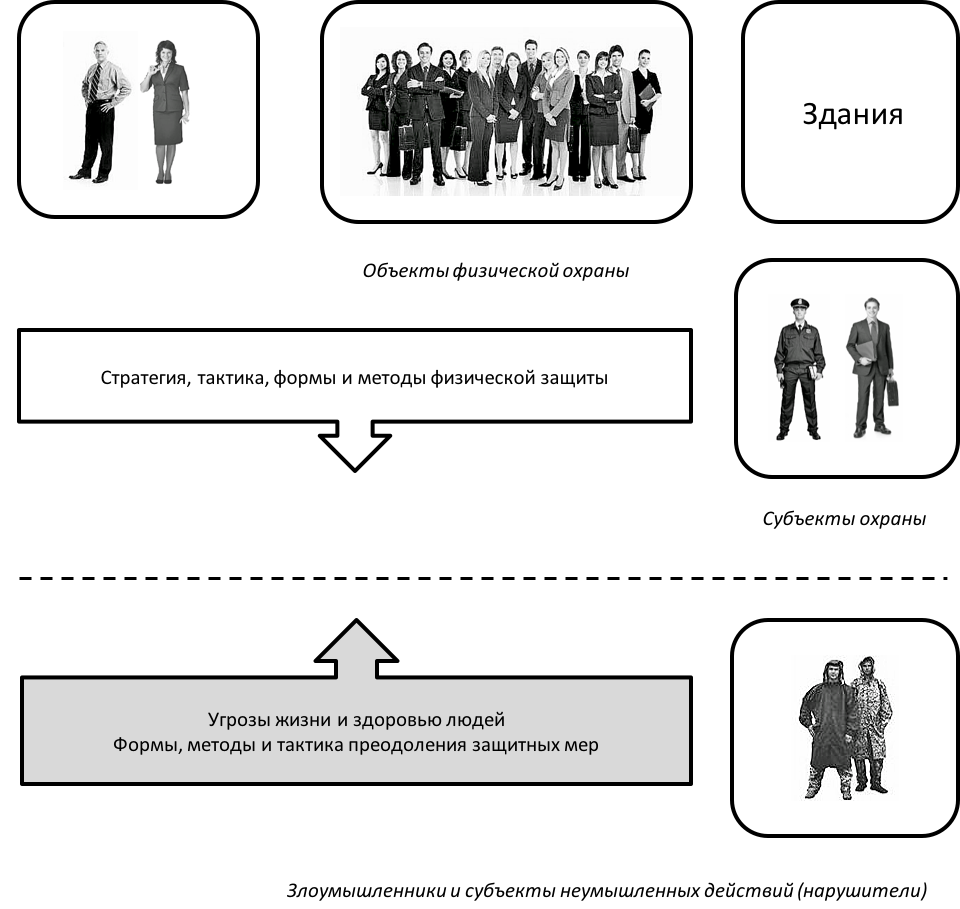
\includegraphics[scale=0.7]{img1}
	\caption{Угроза и защита в области обсепечения физической безопасности}
	\label{image1}
\end{figure}

К \textit{объектам физической охраны} относятся:
\begin{itemize}
	\item Собственники бизнеса и члены их семей;
	\item Топ-менеджеры и персонал предприятия, места их нахождения;
	\item Товарно-материальные и финансовые ценности;
	\item Служебная документация, составляющая коммерческую и иную тайну, а также объекты интеллектуальной собственности;
	\item Объекты недвижимости, а также объекты обеспечения жизнедеятельности предприятия (энергообеспечение, теплоснабжение, водоснабжение и др.).
\end{itemize}

Как правило, объектами физического насилия стано­вятся руководители предприятий или сотрудники, зани­мающие определенное должностное положение (принимают управленческие и кадровые решения, имеют право подписи финансовых документов, участвуют в пла­нировании работы предприятия, заключении сделок, ин­вестиционных проектах и пр.). Вместе с тем, отдельные сотрудники могут становиться объектами физических посягательств и в силу различных конфликтных ситуаций.\\

\begin{tcolorbox}[colback=blue!55!red!5!,colframe=blue!55!red,enforce breakable,% use only breakable in the real world!
	pad at break=1mm, title=Кейс 28. Действия обиженного сотрудника]
	
7 ноября 2012 г. юрист Дмитрий Андреевич Виноградов, 1983 года рождения приехал на работу в компанию «Ригла» (г. Москва) с рюкзаком, в котором находилось специальное снаряжение и боеприпасы, и двумя ружейными чехлами, в которых находились карабины «Сайга» и «Benelli».

В головном офисе фармацевтической компании он беспрепятственно прошел пост охраны, включая металлодетектор. Зашел в мужской туалет на 3-м этаже, где переоделся в военизированный костюм, расчехлил и подготовил к стрельбе оружие. По дороге с третьего на четвертый этаж Виноградов встретил случайно проходившего сотрудника компании и расстрелял его. Затем он прошел к кабинету № 400 и эффектно вошел туда с двумя карабинами наперевес, где начал расстреливать всех присутствовавших. На месте им было убито 4 человека (двое мужчин и две женщины). Двое тяжело раненных лиц были доставлены в клинику, где один из потерпевших скончался от полученных ранений в грудную клетку. Силами службы безопасности «Риглы» Виноградов был задержан и обезоружен. По предварительным данным следствия, он совершил преступление на почве неразделенной любви, а жертвами стали коллеги любимой девушки, которые иронично относились к чувствам Виноградова. К убийству нескольких человек преступник готовился практически год. В это время он не только купил длинноствольное оружие и посещал стрелковый клуб, но и обращался к психиатру с жалобой на проблемы с психикой. 

Начальник охраны «Риглы» был уволен, но это не помогло вернуть к жизни погибших.

\begin{itemize}
	\item[{\color{blue!55!red}\Huge {  $ ? $}} \quad]   Сообщите свое мнение о том, как можно было предотвратить преступление.
\end{itemize}	
	
\end{tcolorbox}

В общем плане к угрозам физической безопасности личности относятся: 
\begin{itemize}
	\item Похищения и угрозы похищения сотрудников, членов их семей и близких родственников; 
	\item Убийства, сопровождаемые насилием, издевательствами и пытками; 
	\item Психологический террор, угрозы, запугивание, шантаж, вымогательство; 
	\item Нападение с целью завладения денежными средствами, ценностями и документами. 
\end{itemize}

Основными способами реализации указанных угроз, как правило,  являются следующие\footnote{Ворона В.А., Тихонов В.А. Концептуальные основы создания и применения системы защиты объектов. М.: Горячая линия – Телеком, 2012. С 28-29}:
 
\begin{itemize}
	\item Взрывы, в том числе с использованием взрывных ус­тройств, снабженных механизмами дистанционного уп­равления; 
	\item Обстрелы  из автоматического  оружия различных калибров, в том числе с использованием специальных при­способлений для ведения снайперской стрельбы в любое время суток; 
	\item Поджоги, в том числе с использованием канистр и иных емкостей с легко воспламеняющимися жидкостями и смесями; 
	\item Акты вандализма, повреждение входных дверей, ре­шеток, ограждений, витрин, а также личных и служебных транспортных средств; 
	\item Ограбления   и   разбойные   нападения   на   офисы, склады и транспортные средства,  перевозящие ценные грузы; 
	\item Налеты на квартиры руководителей компаний или сотрудников фирм; 
	\item Умышленные и заказные убийства; 
	\item Захват заложников; 
	\item Физическое насилие в отношении отдельных со­трудников фирм или членов их семей;
	\item Шантаж, угрозы физического насилия или убий­ства. 
\end{itemize}

В качестве основных мер обеспечения физической безопасности объектовая охрана, организация внутриобъектового и пропускного режимов, мониторинг внешней и внутренней среды охраняемого объекта, личное сопровождение охраняемых лиц, обеспечение режима конфиденциальности маршрутов их передвижения, конкретных мест посещения и мест жительства, отработка стандартных и проверочных маршрутов при передвижении охраняемых лиц.\\

\begin{tcolorbox}[colback=blue!55!red!5!,colframe=blue!55!red,enforce breakable,% use only breakable in the real world!
	pad at break=1mm, title=Кейс 29. Инциденты при охране физических лиц]

30 марта 1981 г. президент США Рональд Рейган вышел из гостиницы «Хилтон» и направился в сторону ожидавшей его автомашины. В это время из толпы вышел Джон Хинкли, выхватил револьвер и, удерживая оружие двумя руками, направил его на президента. Охрана среагировала мгновенно. Один из телохранителей бросился на преступника и сбил его с ног еще до того, как Хинкли успел выстрелить первый раз. До того, как успел нажать на спусковой крючок! А ведь это был выстрел в упор. Другой телохранитель, прикрывая своим телом президента, сгреб его в охапку и втолкнул в бронированный лимузин. Все это заняло менее трех секунд. Однако душевнобольной Хинкли оказался неплохим стрелком. За три секунды в падении он сумел сделать шесть выстрелов. Только последняя пуля попала в автомобиль и рикошетом - в грудь Рейгана! Семидесятилетний президент США остался жив благодаря опыту и самоотверженности личных телохранителей, оказавшихся эффективными на последнем рубеже защиты охраняемого лица. 

28 сентября 2012 г. во время праздничного мероприятия по случаю открытия моста в Храставе на Либерецах к проходившему в толпе президенту Чехии Вацлаву Клаусу приблизился молодой человек в защитном полувоенном костюме. Он достал из кармана пистолет и произвел в упор несколько имитационных выстрелов в правую руку и бок президента. Все произошло настолько быстро, что никто не смог помешать нападавшему. Стрелявший повернулся и спокойно ушел с места происшествия. Телохранители Вацлава Клауса не только отстали на маршруте от охраняемого лица, но и, как оказалось, просто были не готовы к действиям в данной ситуации. Никто не смог задержать покушавшегося и даже не попытался это сделать. Нападавшим оказался 26-летний местный рабочий Павел Вондроуш. Перед задержанием он еще успел спокойно выкурить сигарету и дать интервью подоспевшим журналистам. Свой поступок он объяснил как протест против политиков, которые не замечают простой народ. Намерений навредить Клаусу у него, якобы, не было, т.к. пистолет был игровым. Однако у президента от выстрелов пластиковыми пулями остались синяки, а рубашка оказалась испачкана кровью. Комиссия констатировала, что со стороны охраны имел место профессиональный провал, полное фиаско. Начальник охраны Иржи Скленка подал в отставку.

\begin{itemize}
	\item[{\color{blue!55!red}\Huge {  $ ? $}} \quad]   Проведите сопоставительный анализ действий охраны президентов США и Чехии.
\end{itemize}	

\end{tcolorbox}

Личная охрана должна соответствовать образу жизни охраняемого лица, отличаться решительностью, эффективностью и не броскостью, быть хорошо информированной и уметь хранить конфиденциальную информацию. Сотрудники личной охраны должны быть профессионалами, во время работы не отвлекаться на сторонние вопросы и действовать на упреждение. Своим поведением они не должны давать повода для агрессии. В критических ситуациях сотрудники личной охраны должны быть готовы к самопожертвованию. Руководители охраны обязаны знать, что профессиональные киллеры составляют досье на объекта покушения, изучают маршруты передвижения, места жительства и работы на уязвимость, определяют места и способы покушений.

В целях предупреждения совершения противоправных действий на объектах, специалисты рекомендуют категорировать их на \textit{особо важные, особо режимные, режимные} и \textit{не режимные объекты}. Внутри объекта, в зависимости от его категории, рекомендуют выделять несколько зон безопасности (см. рисунок \ref{image2}). В каждой из указанных на рисунке зон устанавливается свой режим безопасности, связанный с особенностями мер по разграничению доступа сотрудников предприятия и сторонних посетителей. Как правило, в зонах устанавливаются предназначенные для них специальные технические средства. В отдельных зонах комплексно применяют физическую охрану и технические средства. Иногда на периферии устанавливается контрольное оборудование, а управление им осуществляется людьми из центра мониторинга.

\begin{figure}[h]
	\centering
	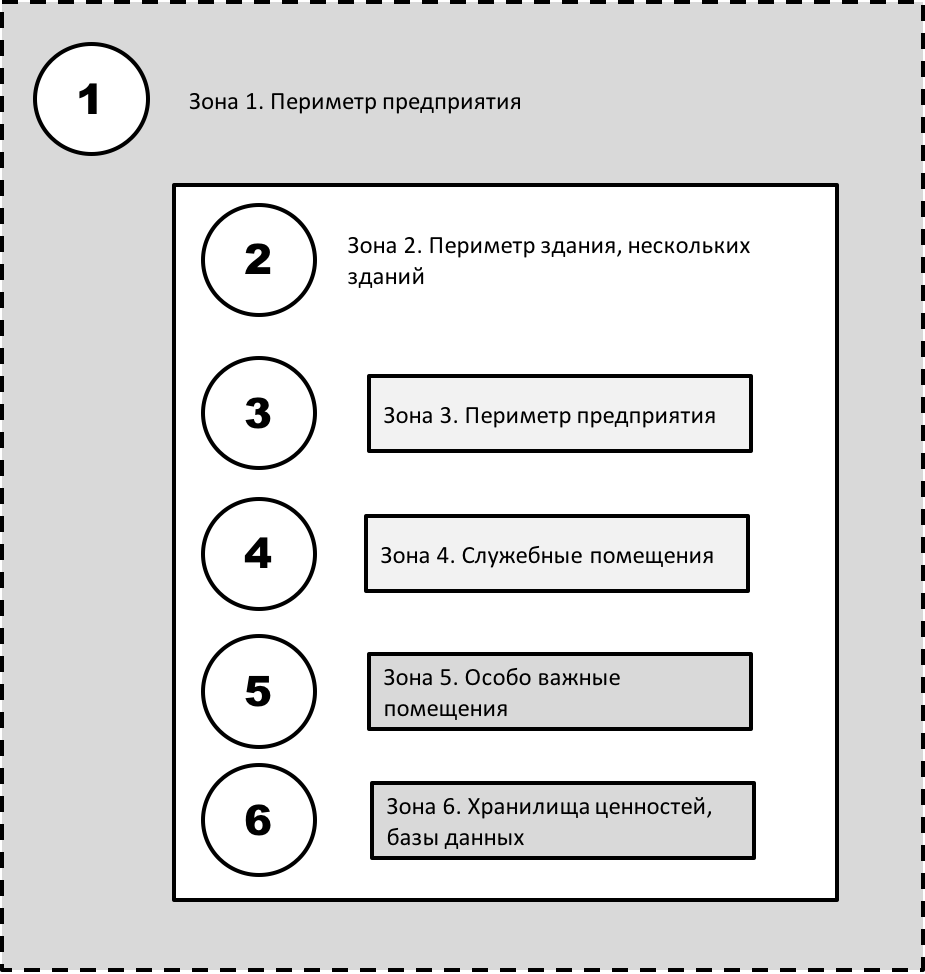
\includegraphics[scale=0.6]{img2}
	\caption{Зоны безопасности внутри объекта по В.А. Вороне и В.А. Тихонову}
	\label{image2}
\end{figure}

В качестве основных \textit{групп причин угроз безопасности личности}, как правило, указывают следующие:
\begin{itemize}
	\item Недобросовестная конкуренция (устранение конкурента);
	\item Действия криминальных сообществ, организаций и преступных групп; 
	\item Попытки добропорядочных граждан решать свои экономические проблемы за счет богатых друзей, знакомых и родственников;
	\item Противоправное урегулирование финансовых конфликтов (расправы с ненадежными партнерами, неплательщиками крупных долгов, устранение кредиторов);
	\item Сокрытие фактов коррупции, устранение свидетелей других преступных действий.
\end{itemize}

\subsection{Угроза сохранности финансов и иных материальных ценностей предприятия}

Субъекты предпринимательской деятельности осуществляют операции с наличными и безналичными денежными средствами, иными материальными ценностями. Данные средства, обладающие существенным стоимостным выражением, бывают представлены в виде: 
\begin{itemize}
	\item Российской и иностранной наличной и безналичной валюты; ценных бумаг; 
	\item Подлинников правоустанавливающих документов; драгоценных и полудрагоценных камней;
	\item Драгоценных металлов и изделий из камней и металлов;
	\item Дорогостоящего движимого имущества; 
	\item Произведений искусства, антикварных ценностей и др. 
\end{itemize}
	
Указанные предметы и документы всегда являлись объектом покушения злоумышленников и, в этой связи, всегда охранялись (см. рисунок \ref{image3}).

С учетом того, что материальные и иные ценности носят разный характер, а также выполняют различные функции на различных этапах производства, злоумышленники вырабатывают различные методы завладения защищаемыми объектами, а физическая охрана постоянно совершенствует меры защиты. К примеру, драгоценные металлы и камни являются объектами четко регламентированной физической защиты на всех этапах производственной цепочки: добыча (производство), обогащение, обработка (включая огранку), производство продукции для целей науки, техники и личного потребления. Это делается осознанно – на всех стадиях драгоценные металлы и камни являются объектами преступных посягательств. Субъектами противоправной деятельности могут быть сторонние лица, работники предприятий отрасли и даже работники охраны. По этой причине защитные меры должны носить комплексный характер, быть сбалансированными и предусматривать применение принципа «не менее двух ключей».

В отрасли по добыче и переработке природных нефти и газа также на всех этапах технологической цепочки сложились традиционные методы хищения энергоносителей. Как правило, наибольшие объемы незаконного отъема совершаются в процессе перекачки нефти и газа по трубопроводным магистралям. К примеру, сразу после распада Советского Союза в 1991 г., украинские юридические лица приступили к несанкционированному отбору (хищению) газа, поступавшего из России транзитом через территорию Украины в страны западной Европы. Злоумышленники использовали особенность конструкции трубопроводных систем в рамках единой страны (СССР), что не позволяло с территории Российской Федерации в полной мере контролировать действия компании «Укртрансгаз» и связанных с ней должностных лиц. 

\begin{figure}[h]
	\centering
	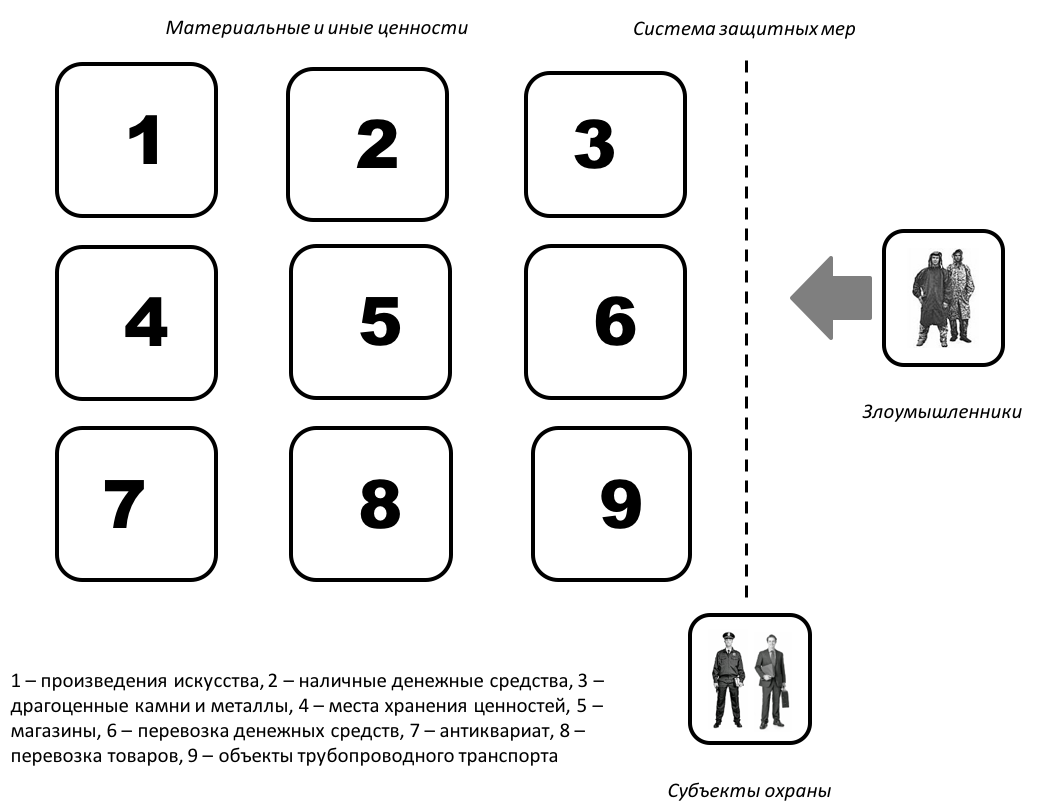
\includegraphics[scale=0.7]{img3}
	\caption{Принципиальная схема физической зашиты ценностей откорыстных посягательств}
	\label{image3}
\end{figure}

На объектах трубопроводного транспорта, связанных, прежде всего, с перекачкой нефти, нефтепродуктов и природного газа, распространенным явлением является хищение путем несанкционированной врезки в магистральный трубопровод. При этом в последнее время наиболее часто подобный метод используется в удаленных местностях, путем осуществления врезки под землей и под водой, с другими ухищрениями, осложняющими поиск и выявление неправомерных действий злоумышленников.

Основные угрозы сохранности материальных ценностей предприятия реализуются, как правило, в следующих основных формах:
\begin{itemize}
	\item Деятельность преступных групп, конкурирующих экономических структур, а также отдельных лиц, занимающихся противоправными действиями в отношении собственности, которые могут привести к значительным материальным и финансовым потерям организации или ее отдельным подразделениям.
	\item Непреднамеренные (ошибочные, случайные, необдуманные, без корыстных целей) нарушения установленных требований учета, хранения, оборота, правил торговли товарно-материальных ценностей, финансовых ресурсов, служебных документов и информации, приводящие к непроизводительным затратам ресурсов, утратам и хищениям.
	\item Преднамеренные (в корыстных целях, по принуждению, со злым умыслом, т.п.) действия сотрудников компании, допущенных к материальным, финансовым и информационным ресурсам:
	\begin{itemize}
		\item Различные виды хищений товарно-материальных ценностей отдельными сотрудниками или в сговоре на объектах организации;
		\item Умышленное нарушение денежно-кассовых операций с клиентами, поставщиками продукции, повлекшее недостачи;   
		\item Подделка учетных и отчетных документов хранения и оборота товарно-материальных ценностей;
		\item Хищение носителей конфиденциальной информации (распечаток, магнитных дисков, запоминающих устройств) для использования в личных корыстных целях.
	\end{itemize}
	\item Отказы и сбои в работе инженерно-технических средств охраны (систем СКУД, ОПС, видеонаблюдения и связи), приводящие к непроизводительным затратам:
	\begin{itemize}
		\item отключение электричества в офисе и на объектах предприятия;
		\item незапланированная потеря каналов связи, невозможность управления системой охранно-пожарной сигнализации и видеонаблюдения на объектах с пульта централизованного наблюдения;
		\item нарушение функционирования пульта централизованного наблюдения у оперативного дежурного (некомпетентность оператора, сбой программного обеспечения, выход из строя отдельных комплектующих компьютера, др.);
		\item выход из строя системы видеонаблюдения на объектах компании, вследствие чего допущены непроизводственные потери материальных и финансовых средств;
		\item нарушение работы системы СКУД, несанкционированный пропуск посторонних лиц на территорию объектов компании, допуск к товарно-материальным ценностям, конфиденциальной информации.
	\end{itemize}
	\item Аварии, техногенные катастрофы и природные катаклизмы.
\end{itemize}

Отдельную сферу угроз финансовым и материальным ценностям составляют угрозы в сфере инкассации. Они также носят как внешний, так и внутренний характер. Инкассация является специализированной сферой банковской деятельности и по этой причине лицензируется Банком России и его территориальными учреждениями. С другой стороны, инкассация выражается в перемещении наличных денежных средств и иных материальных ценностей под охраной. По этой причине в своей деятельности инкассация использует оружие, боеприпасы и специальные средства.  Одной из важнейших внутренних задач является обеспечение кадровой безопасности службы инкассации.\\


\begin{tcolorbox}[colback=blue!55!red!5!,colframe=blue!55!red,enforce breakable,% use only breakable in the real world!
	pad at break=1mm, title=Кейс 30. Чрезвычайное происшествие в Перми]
	
29 июня 2009 г. в Перми было совершено разбойное нападение на автомобиль инкассации Западно-Уральского банка ОАО «Сбербанк России». В результате данного преступления было похищено 250 000 000 руб. наличными\footnote{Сайт «Википедия» [Электронный ресурс], информационно-справочный портал. М. URL: https: //ru.wikipedia.org (дата обращения: 24.02.2015 г.)}. По факту было возбуждено уголовное дело и начаты оперативно-розыскные мероприятия. В результате было установлено, что автомашина инкассации с крупной суммой наличных денежных средств направлялась в рассчетно-кассовый центр банка. Старший инкассатор Шуман А.В., угрожая огнестрельным оружием своим коллегам, заставил их заехать вглубь лесного массива и остановить там автомобиль. После этого злоумышленник запер инкассаторов в бронированной кабине автомобиля и перегрузил мешки с деньгами в поджидавший его легковой автомобиль и скрылся в неизвестном направлении. Принятыми мерами Шуман А.В. и другие участники преступной группы были обнаружены и задержаны. Организатор преступления указал на место нахождения тайника с похищенными деньгами. В банк была возвращена практически вся сумма, исключением 1 145 000, 300 руб. уже потраченных преступниками. Во время следствия было установлено, что Шуман А.В. более 12 лет работал инкассатором и был на хорошем счету. К преступлению он готовился два года. В качестве побуждающего мотива бывший инкассатор сослался на сложную, опасную и мало оплачиваемую работу. 10 февраля 2010 г. судом Шуман А.В. был признан виновным в совершении ограбления и приговорен к восьми годам лишения свободы в исправительной колонии строгого режима. Трое соучастников описанного преступления были также привлечены к уголовной ответственности.	

\begin{itemize}
	\item[{\color{blue!55!red}\Huge {  $ ? $}} \quad]   Предложите меры по предотвращению корыстных преступлений со стороны инкассаторов.
\end{itemize}	
	
\end{tcolorbox}
	
Еще больше рисков возникает при инкассации ценностей не уполномоченными на то лицами. «Серые» схемы инкассации производятся с участием частных охранных предприятий и даже работников полиции, которые не имеют соответствующей лицензии Банка России. В ряде случаев подобные бригады инкассаторов имеют даже табельное оружие, однако они не имеют необходимой профессиональной подготовки и часто становятся жертвами нападений преступников. В некоторых организациях допускаются «черные» схемы инкассации, когда в качестве курьеров для перевозки денежных средств используются собственные штатные работники – бухгалтера и водители. Руководители предприятий, которые таким образом пытаются минимизировать расходы. В ряде случаев это приводит не только к безвозвратной потере крупных сумм денежных средств, но и к гибели людей, давших согласие эти средства перевозить. Отдельные работники коммерческих банков даже пытаются путем нарушения правил совершения валютно-денежных операций и правил инкассации, разрабатывать схемы зарабатывания средств на обменных операциях, игнорируя всевозможные угрозы. В таких ситуациях к операционным искам добавляются риски контрагентов и весьма реальные риски потери деловой репутации.\\
	
\begin{tcolorbox}[colback=blue!55!red!5!,colframe=blue!55!red,enforce breakable,% use only breakable in the real world!
	pad at break=1mm, title=Кейс 31. Изобретательный менеджер]

20 сентября 1999 г. коммерческий банк «Первое общество взаимного кредита» в процессе совершения валютно-обменной операции утратил наличные денежные средства в сумме свыше 250 000 долларов США. Проведенное по факту служебное расследование позволило установить, что материальный ущерб банку был нанесен в результате действий первого заместителя председателя правления данного финансового учреждения, которого мы назовем «Першин». Неправильно трактуя свои должностные полномочия и игнорируя требования действующего законодательства, руководитель на регулярной основе осуществлял «черные схемы» валютно-обменных операций. Каждое утро «Першин» лично обзванивал пункты обмена валюты столичного города и составлял схему из нескольких операций в целях получения определенной прибыли от каждой. После этого по его указанию из хранилища банка изымали часть наличных денежных средств, их складывали в личные автомобили работников казначейства банка, которые объезжали несколько обменных пунктов. При этом сотрудники казначейства, боясь потерять работу, шли на выполнение поручений, но перед выездом даже прощались с коллегами, понимая рискованность ситуации. При совершении последней операции они передали 250 000 долларов «кассиру» обменного пункта, который закрыл шторку окна под предлогом пересчета. Работники банка прождали около часа, стали стучаться в окно пункта и, в конечном итоге, установили, что работники обменного пункта исчезли вместе с деньгами. Служебное расследование также показало, что по указанию «Першина» было проведено более 20 подобных операций, прибыль от которых в общем итоге составила 74 тыс. рублей. Последняя операция нанесла ущерб банку, перекрыв на несколько порядков полученный ранее сомнительный доход.	
	
\begin{itemize}
	\item[{\color{blue!55!red}\Huge {  $ ? $}} \quad]   Опишите банковские нормативы, которые возможно были нарушены менеджером.
\end{itemize}	
	
\end{tcolorbox}	
	
	
\subsection{Угроза сохранности объектов недвижимости}	
	
Здания, сооружения и иное недвижимое имущество относятся к основным средствам предприятия. Как правило, они являются дорогостоящими объектами собственности, требующими постоянного вложения средств в текущие и капитальные ремонты, переоборудование. Недвижимость также подлежит страхованию, и она же является объектом налогообложения. В то же время недвижимость может быть гарантией внешних обязательств предприятия, считается «твердым» залогом при получении кредитов, является подтверждением реальной производственной деятельности.

Естественно, что объекты недвижимости подвержены рискам. Некоторые из них носят объективный характер – природоестественные, техногенные и экологические катастрофы, неблагоприятные политические факторы, включая масштабные войны и локальные вооруженные конфликты. Многие риски связаны с умышленными или неумышленными действиями людей и носят субъективный характер. Тем не менее, подобные конфликты также могут нанести существенный ущерб. Любое предприятие, владеющее объектами недвижимости, должно умело защищать их от рисков (см. рисунок \ref{image4}).

\begin{figure}[h]
	\centering
	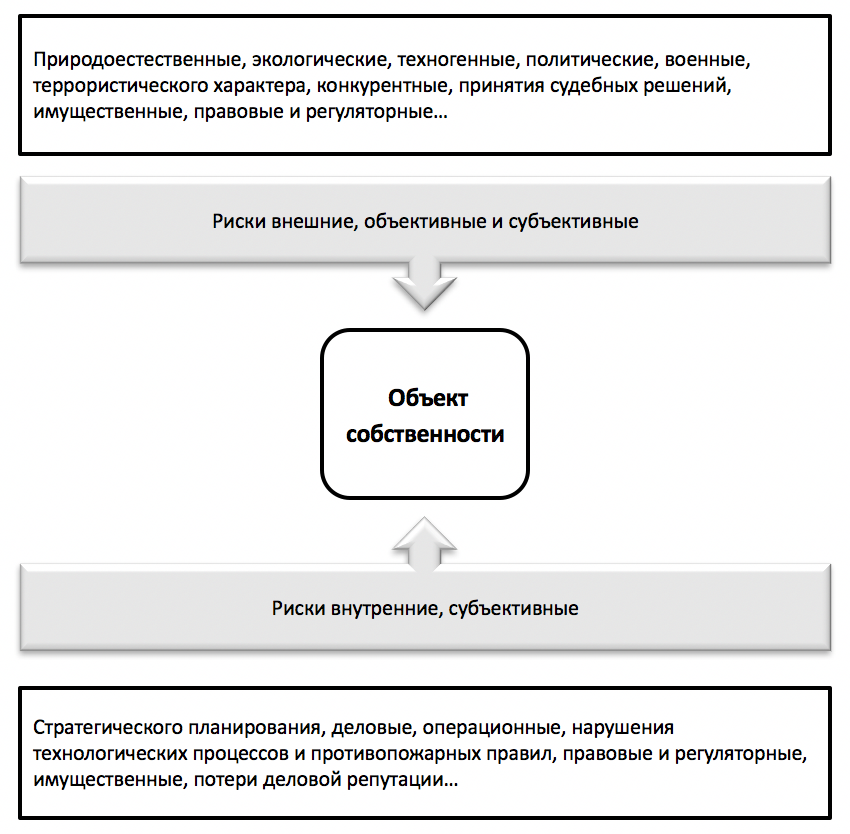
\includegraphics[scale=0.7]{img4}
	\caption{Риски и угрозы сохранности объектов собственности}
	\label{image4}
\end{figure}

Как следует из размещенного выше рисунка, риски сохранности объектов недвижимости могут быть внешними и внутренними, могут носить объективный и субъективный характер. Часть внешних рисков может минимизироваться путем страхования и перестрахования имущества. Однако возможную реализацию некоторых рисков этой категории сложно спрогнозировать заранее. К примеру, весной 2013 г. сложно было предположить, что на Украине произойдет государственный переворот, который повлечет за собой смену власти, силовой передел собственности, локальные вооруженные конфликты, повлекшие за собой массовую гибель людей, уничтожение промышленных объектов и инфраструктуры.

С учетом этих особенностей преступные посягательства на здания и помещения в отдельных регионах из категории потенциальных рисков переходят в категорию рисков реальных, угроза возникновения которых становится весьма вероятной:
\begin{itemize}
	\item Взрывов;
	\item Обстрелов из огнестрельного оружия;
	минирования, в том числе с применением дистанционного управления;
	\item Поджогов;
	\item Нападения, вторжения, захватов, пикетирования, блокирования;
	\item Повреждения входных дверей, решеток, ограждений, витрин, мебели, а также транспортных средств личных и служебных;
	\item Технологические аварии, пожары.
\end{itemize}

Целями подобных акций могут быть нанесение серьезного материального и морального ущерба, срыв на длительное время нормального функционирования объектов, вымогательство значительных сумм денег или каких-либо льгот (кредиты, отсрочка или погашение платежей и т. п.) перед лицом террористической угрозы. В зонах локальных вооруженных конфликтов такие цели могут быть вызваны исключительно военными соображениями. По мнению некоторых специалистов\footnote{Люттвак Э.Н. Стратегия: логика войны и мира. М.: Университет Дмитрия Пожарского, 2012. С 149}, чем сильнее акцент на истощение противника в общем стиле войны, тем эффективнее становятся техники обнаружения цели, атаки и снабжения. Такой процесс заменяет собой искусство войны. Всякий раз, когда материально превосходящая сторона способна извергать боевую мощь, она без ограничения наносит удары на позиции противника (окопы, города и иные населенные пункты, объекты промышленности и социальной сферы).

В любом случае следует учитывать, что ряд объектов недвижимости нуждается в повышенных мерах физической защиты от любых внешних и внутренних угроз. К таким особо важным и важным объектам можно отнести предприятия по изготовлению боеприпасов, высокотоксичные производства, объекты атомной энергетики, гидротехнические сооружения, объекты добычи, транспортировки и переработки нефти и газа, места хранения значительных материальных ценностей. Указанные и некоторые другие объекты нормативно категорированы и отнесены к области государственного мониторинга по вопросам противопожарной защиты, гражданской обороны и комплексного обеспечения их безопасности. Физическая охрана таких, равно как и иных объектов может быть отнесена к компетенции различных охранных структур, деятельность которых разрешена в нашей стране.\\	

\begin{tcolorbox}[colback=blue!40!red!1!,colframe=blue!40!red,enforce breakable,% use only breakable in the real world!
	pad at break=1mm, title=Вопросы и задания для самоконтроля]
	\begin{itemize}
		\item[{\color{blue!55!red}\Huge { $ ? $}} ]  Дайте определение понятия «частная охранная деятельность».
		\item[{\color{blue!55!red}\Huge {  $ ? $}} ] Опишите возможные угрозы в области защиты жизни и здоровья физических лиц.
		\item[{\color{blue!55!red}\Huge {  $ ? $}} ] Расскажите об угрозах проникновения посторонних лиц в места хранения материальных ценностей.
		\item[{\color{blue!55!red}\Huge {  $ ? $}} ] Расскажите об угрозах проникновения на охраняемые объекты посторонних лиц, представляющих интересы рейдеров.
		\item[{\color{blue!55!red}\Huge {  $ ? $}} ] Расскажите об угрозах похищения наличных денежных средств и иных материальных ценностей во время их инкассации.		
	\end{itemize}		
\end{tcolorbox}

\section{Организация частной и иной охранной деятельности}

\begin{tcolorbox}[colback=blue!40!red!10!,colframe=blue!40!red]
В результате изучения главы студент должен \textbf{знать} субъектов осуществления различных видов обеспечения физической безопасности в нашей стране, их полномочиях, права и обязанности; \textbf{уметь} выделять особенности организации деятельности ведомственной охраны предприятий и организаций, частных охранных предприятий и военно-охранных компаний, вневедомственной охраны полиции и порядком осуществления государственной охраны высших должностных лиц страны; \textbf{владеть} методами применения на предприятии физической охраны, подходами определения ее состава и направлений взаимодействия внутри системы безопасности, а также расчета экономических затрат на применение различных вариантов физической защиты.
\end{tcolorbox}

\subsection{Порядок создания и функционирования частных охранных предприятия}

В соответствии с действующим законодательством охранную деятельность в нашей стране осуществляют федеральные государственные органы, специально выделенные структурные подразделения министерств, ведомств, организаций и предприятий. Каждый из участников этой деятельности обладает своей сферой компетенции и установленными полномочиями. Ряд указанных структур, а также организации с особыми уставными задачами наделены правом на хранение и применение оружия, патронов к нему и специальных средств. Общую структуру и взаимосвязь государственных органов и иных организаций, осуществляющих охранную деятельность в Российской Федерации, можно представить следующим образом (см. рисунок \ref{image5}). Как правило, функции охранных структур разграничены, однако в ряде случаев некоторые государственные и частные организации конкурируют на рынке услуг безопасности.

\begin{figure}[h]
	\centering
	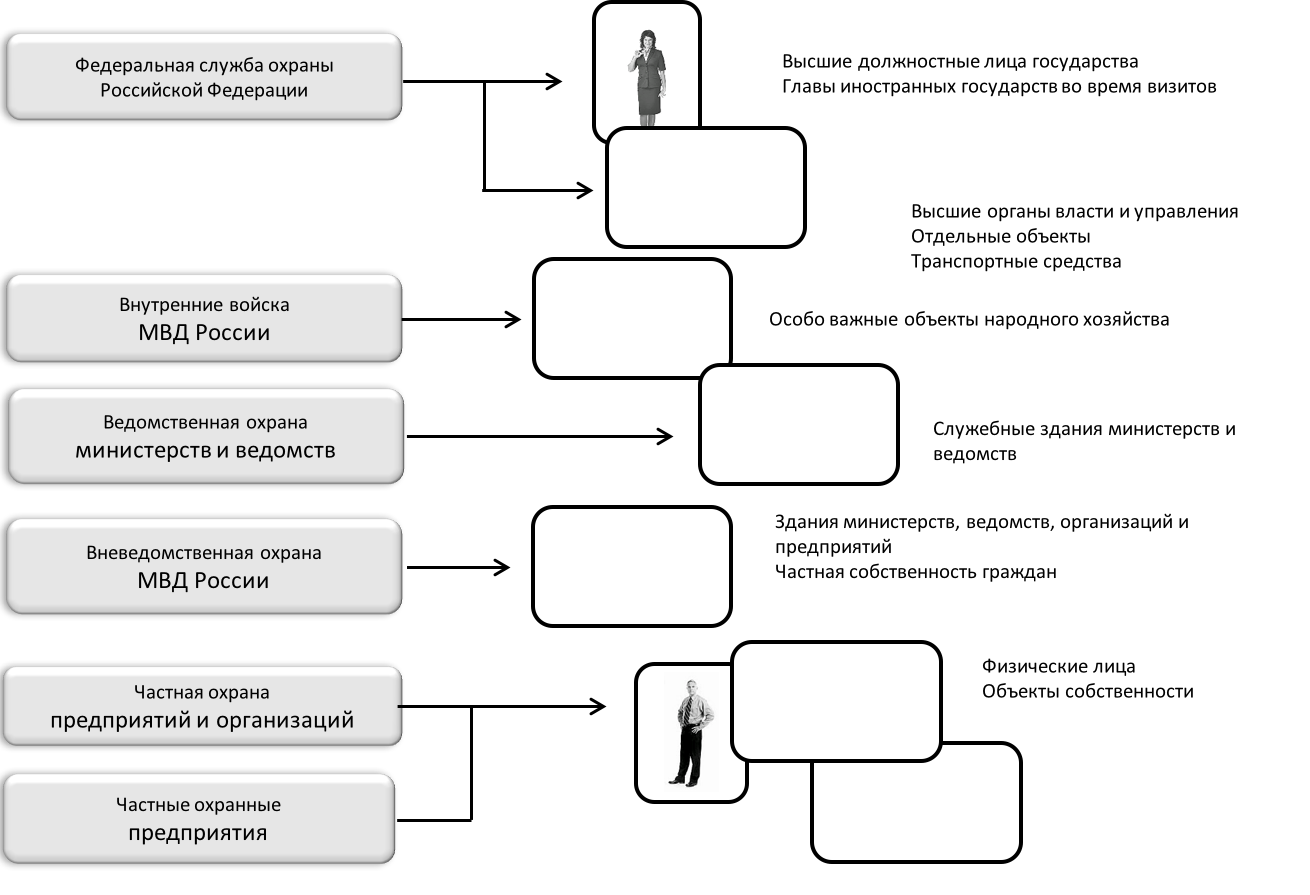
\includegraphics[scale=0.7]{img5}
	\caption{Органы, предприятия и организации, наделенные правом осуществления функция охраны}
	\label{image5}
\end{figure}

Частная охранная деятельность в нашей стране регулируется федеральным законодательством с 1992 г. Соответствующий федеральный закон имеет прямое действие. \\

\definition{Частная охранная деятельность}{оказание на возмездной договорной основе услуг физическим и юридическим лицам имеющими специальное разрешение (лицензию) органов внутренних дел организациями и индивидуальными предпринимателями в целях защиты законных прав и интересов своих клиентов.}

В целях охраны разрешается предоставление следующих услуг:
\begin{itemize}
	\item Защита жизни и здоровья граждан;
	\item Охрана объектов и (или) имущества (в т.ч. при его транспортировке), находящихся в собственности, во владении, в пользовании, хозяйственном ведении, оперативном управлении или доверительном управлении, за некоторыми исключениями;
	\item Охрана объектов и (или) имущества на объектах с осуществлением работ по проектированию, монтажу и эксплуатационному обслуживанию технических средств охраны, перечень видов который устанавливается Правительством Российской Федерации, и (или) с принятием соответствующих мер реагирования на их сигнальную информацию;
	\item Консультирование и подготовка рекомендаций клиентам по вопросам правомерной защиты от противоправных посягательств;
	\item Обеспечение порядка в местах проведения массовых мероприятий;
	\item Обеспечение внутриобъектового и пропускного режимов на объектах;
	\item Охрана объектов и (или) имущества, а также обеспечение внутриобъектового и пропускного режимов на объектах, в отношении которых установлены обязательные для выполнения требования к антитеррористической защищенности, за исключением объектов, подлежащих государственной охране.
\end{itemize}

Как было указано выше, частная охранная деятельность не распространяется на объекты государственной охраны, а также некоторые иные охраняемые объекты, перечень которых утверждается Правительством Российской Федерации. Запрещается вооруженная охрана имущества на территориях закрытых административно-территориальных образований, а также приобретение и использование оружия частными охранными организациями, зарегистрированными и (или) расположенными на их территориях. Оказание охранных услуг в целях защиты объектов транспортной инфраструктуры и транспортных средств от актов незаконного вмешательства осуществляется с учетом требований законодательства о транспортной безопасности.

Право на приобретение правового статуса частного охранника предоставляется гражданам, прошедшим профессиональное обучение для работы в данном качестве и сдавшим квалификационный экзамен. Статус подтверждается выдачей удостоверения частного охранника. Не вправе претендовать на статус частного охранника лица:
\begin{itemize}
	\item Не достигшие восемнадцати лет; признанные решением суда недееспособными или ограниченно дееспособными;
	\item Имеющие заболевания, которые препятствуют исполнению ими обязанностей частного охранника (перечень таких заболеваний устанавливается Правительством Российской Федерации);
	\item Имеющие судимость за совершение умышленного преступления; 
	\item Которым предъявлено обвинение в совершении преступления; 
	\item А также лица, в отношении которых по результатам проверки имеется заключение о невозможности допуска к осуществлению частной охранной деятельности в связи с повышенной опасностью нарушения прав и свобод граждан, возникновением угрозы общественной безопасности. 
	\item К работе частными охранниками также не допускаются лица, досрочно прекратившие полномочия по государственной должности или уволенные с государственной службы, в т.ч. из правоохранительных органов, из органов прокуратуры, судебных органов по основаниям совершения ими дисциплинарных проступков, грубым или систематическим нарушениям дисциплины, совершением проступка, порочащего честь государственного служащего, утратой доверия к нему, если с момента прекращения полномочий (увольнения) прошло менее трех лет. 
\end{itemize}

Уполномоченным органом в области лицензирования частной охранной деятельности являются органы внутренних дел. В МВД России эту деятельность координирует Управление по организации лицензионно-разрешительной работы и соответствующие подразделения территориальных органов. Им предоставлены полномочия по оказанию следующих государственных услуг\footnote{Официальный сайт Министерства внутренних дел Российской Федерации. Управление по организации лицензионно-разрешительной работы [Электронный ресурс] //mvd.ru: информационно-справочный портал. М. URL: https://mvd.ru/mvd/structur1/Upravleni/ulrr/Gosv (дата обращения: 26.02.2015)}:

\begin{itemize}
	\item Прием квалификационного экзамена у граждан, прошедших ранее обучение по программе профессиональной подготовки частных охранников;
	\item Выдача лицензии на частную охранную деятельность;
	\item Выдача удостоверения частного охранника;
	\item Исполнение функции контроля за частной охранной деятельностью;
	\item Выдача юридическим лицам с особыми уставными задачами разрешения на хранение и использование служебного оружия и патронов к нему.
\end{itemize}

В рамках охранного бизнеса первоначально оформляется лицензия юридического лица на право заниматься частной охранной деятельностью. На следующем этапе устанавливается и изучается объект охраны, формируется концепция его защиты, производится расчет требуемых сил и средств, набирается персонал охраны.

%slide20




\end{document}